\chapter{Escenas}

\begin{figure}[H]
	\centering
	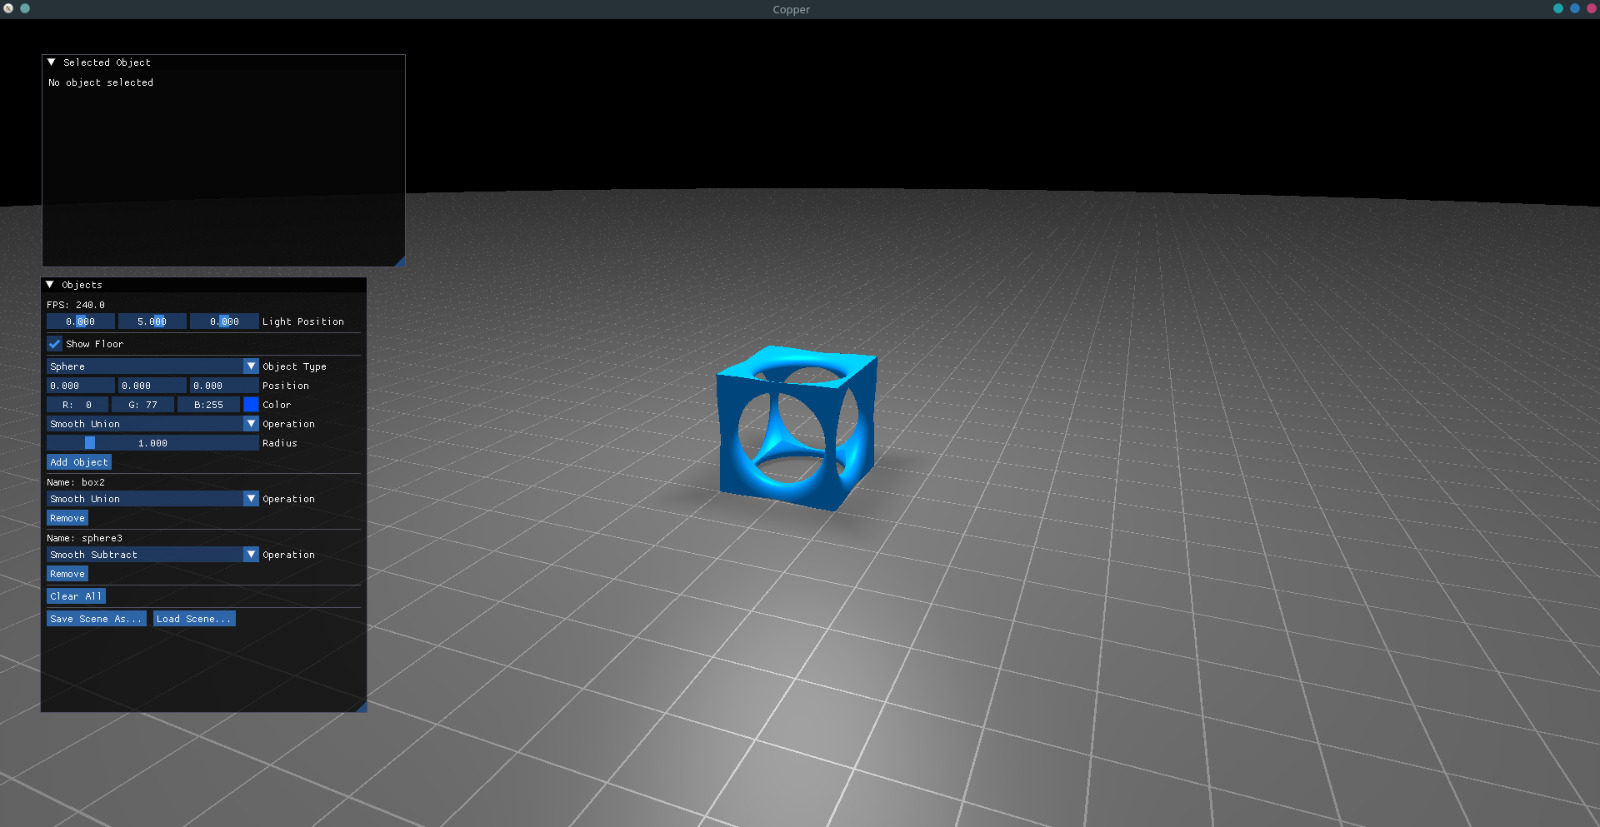
\includegraphics[width=0.7\textwidth]{imagenes/Cubo_esfera.jpg}
	\caption{Combinación de cubo y esfera mediante SDF.}
\end{figure}

\begin{figure}[H]
	\centering
	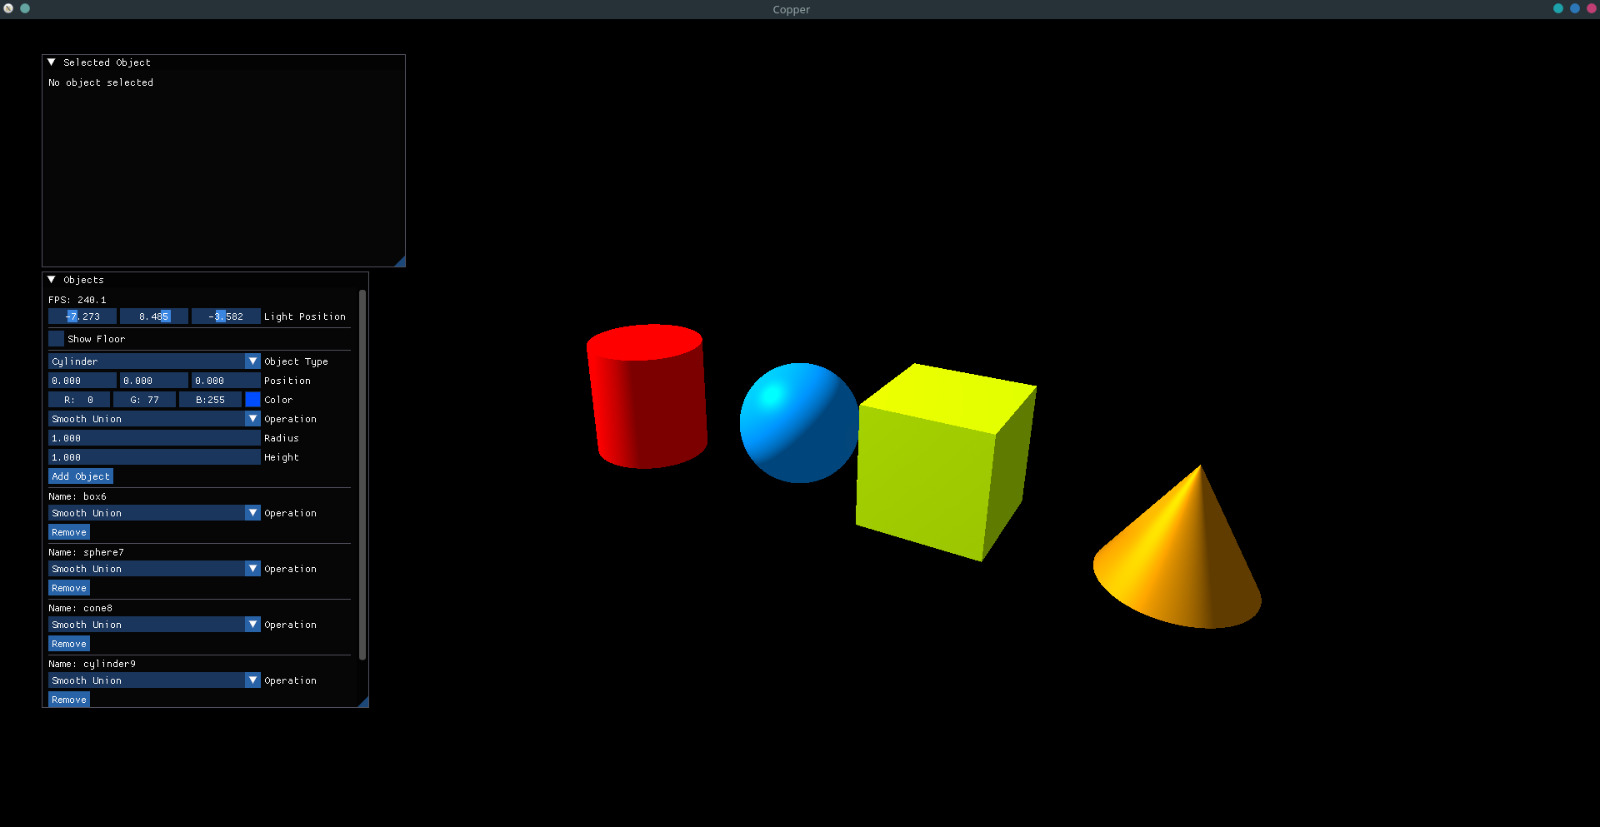
\includegraphics[width=0.7\textwidth]{imagenes/objetos_sin_suelo.jpg}
	\caption{Escena con objetos sin plano de referencia.}
\end{figure}

\begin{figure}[H]
	\centering
	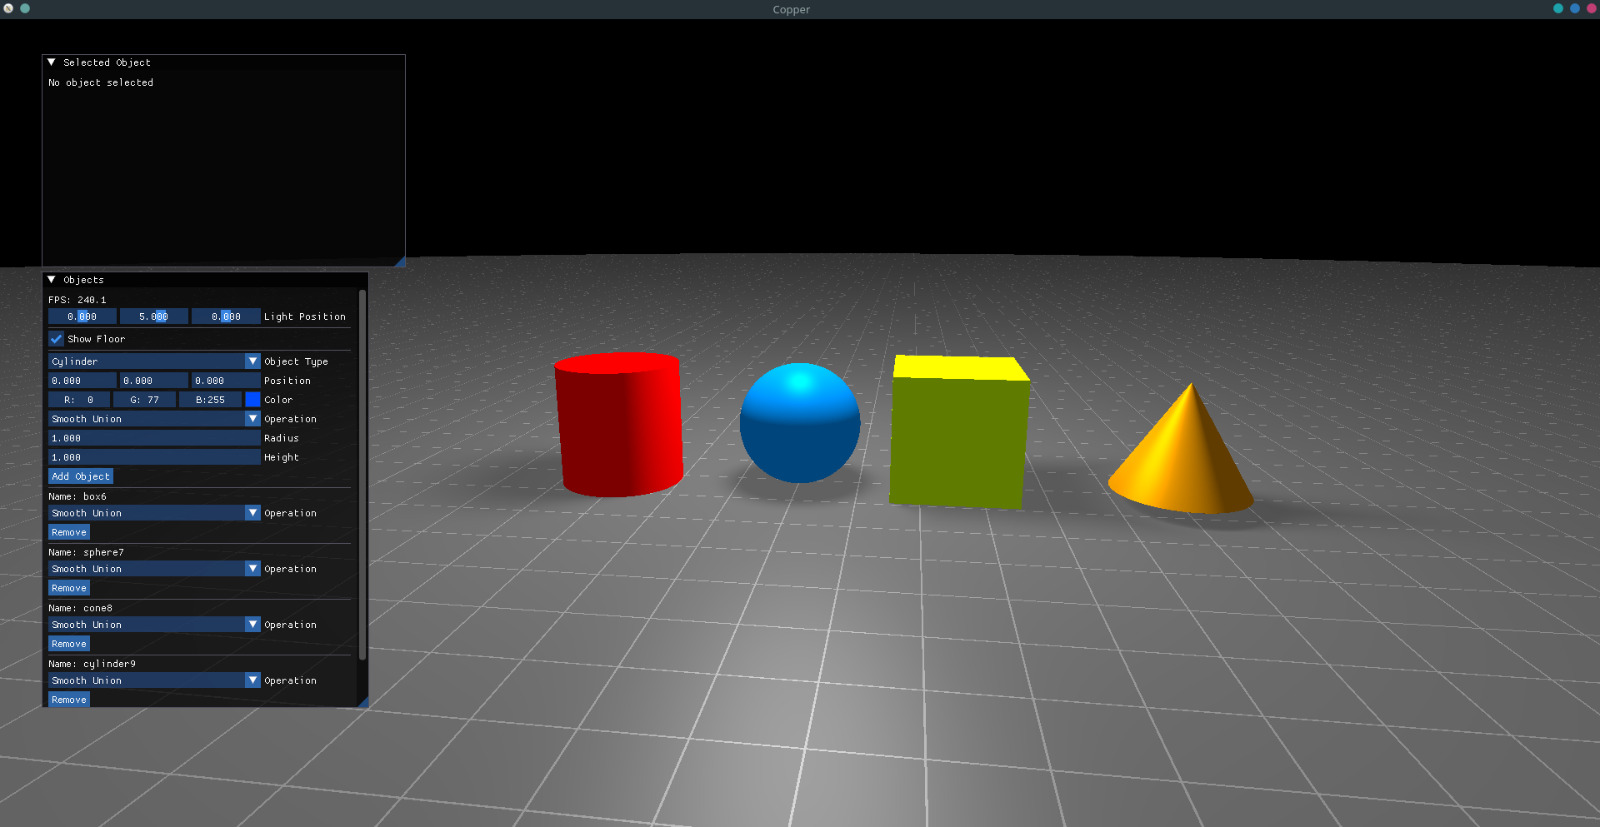
\includegraphics[width=0.7\textwidth]{imagenes/objetos_suelo.jpg}
	\caption{Escena con objetos y plano de referencia activado.}
\end{figure}

\begin{figure}[H]
	\centering
	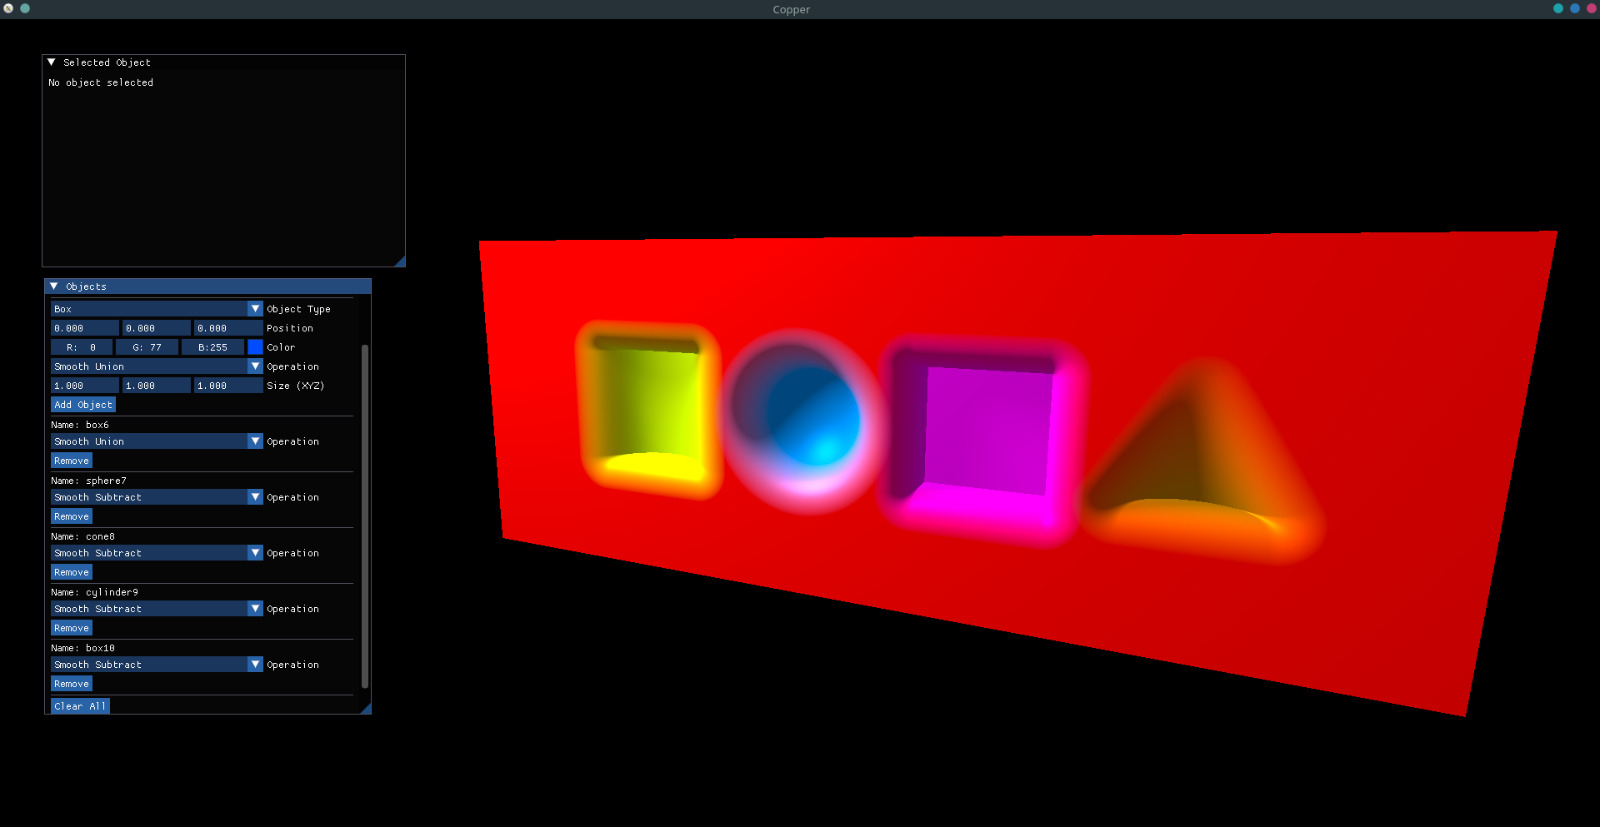
\includegraphics[width=0.7\textwidth]{imagenes/smooth_substract.jpg}
	\caption{Ejemplo de operación smooth subtract entre objetos.}
\end{figure}

\begin{figure}[H]
	\centering
	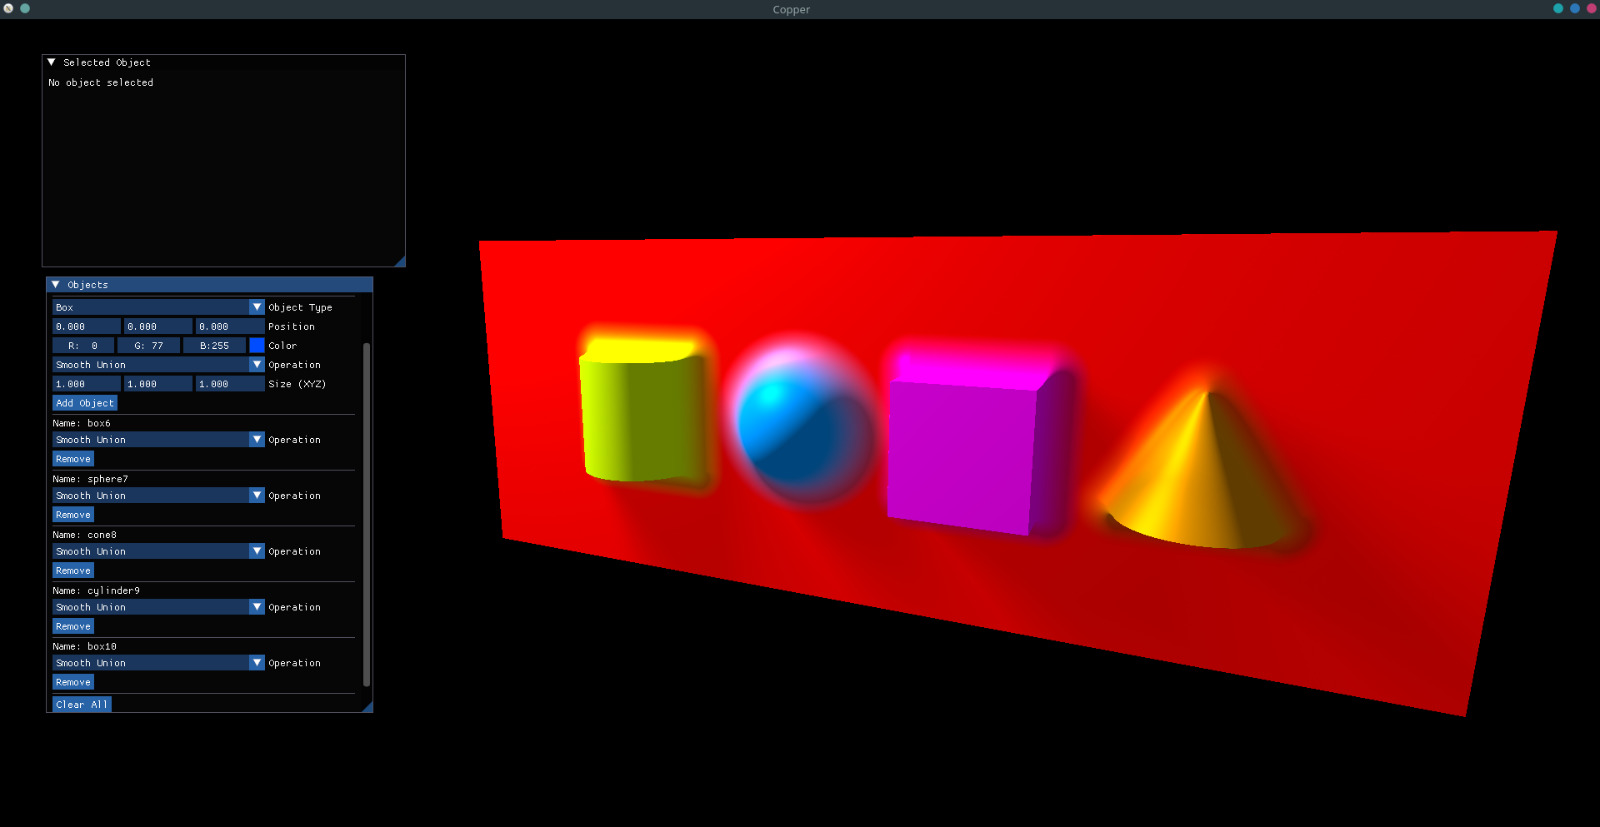
\includegraphics[width=0.7\textwidth]{imagenes/smooth_union.jpg}
	\caption{Ejemplo de operación smooth union entre objetos.}
\end{figure}

\begin{figure}[H]
	\centering
	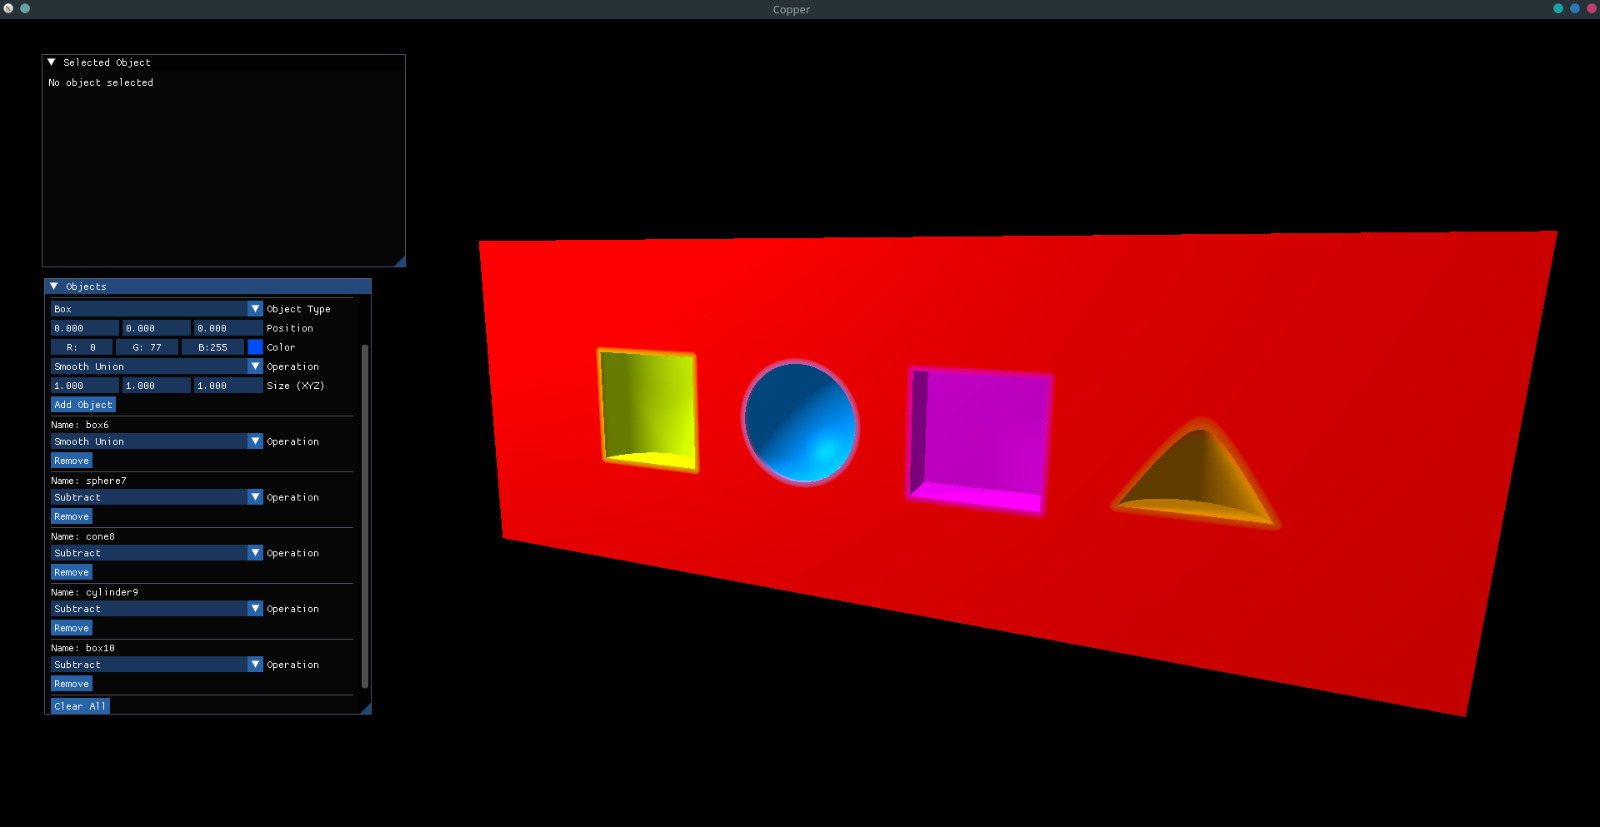
\includegraphics[width=0.7\textwidth]{imagenes/substract.jpg}
	\caption{Ejemplo de operación de sustracción entre objetos.}
\end{figure}

\begin{figure}[H]
	\centering
	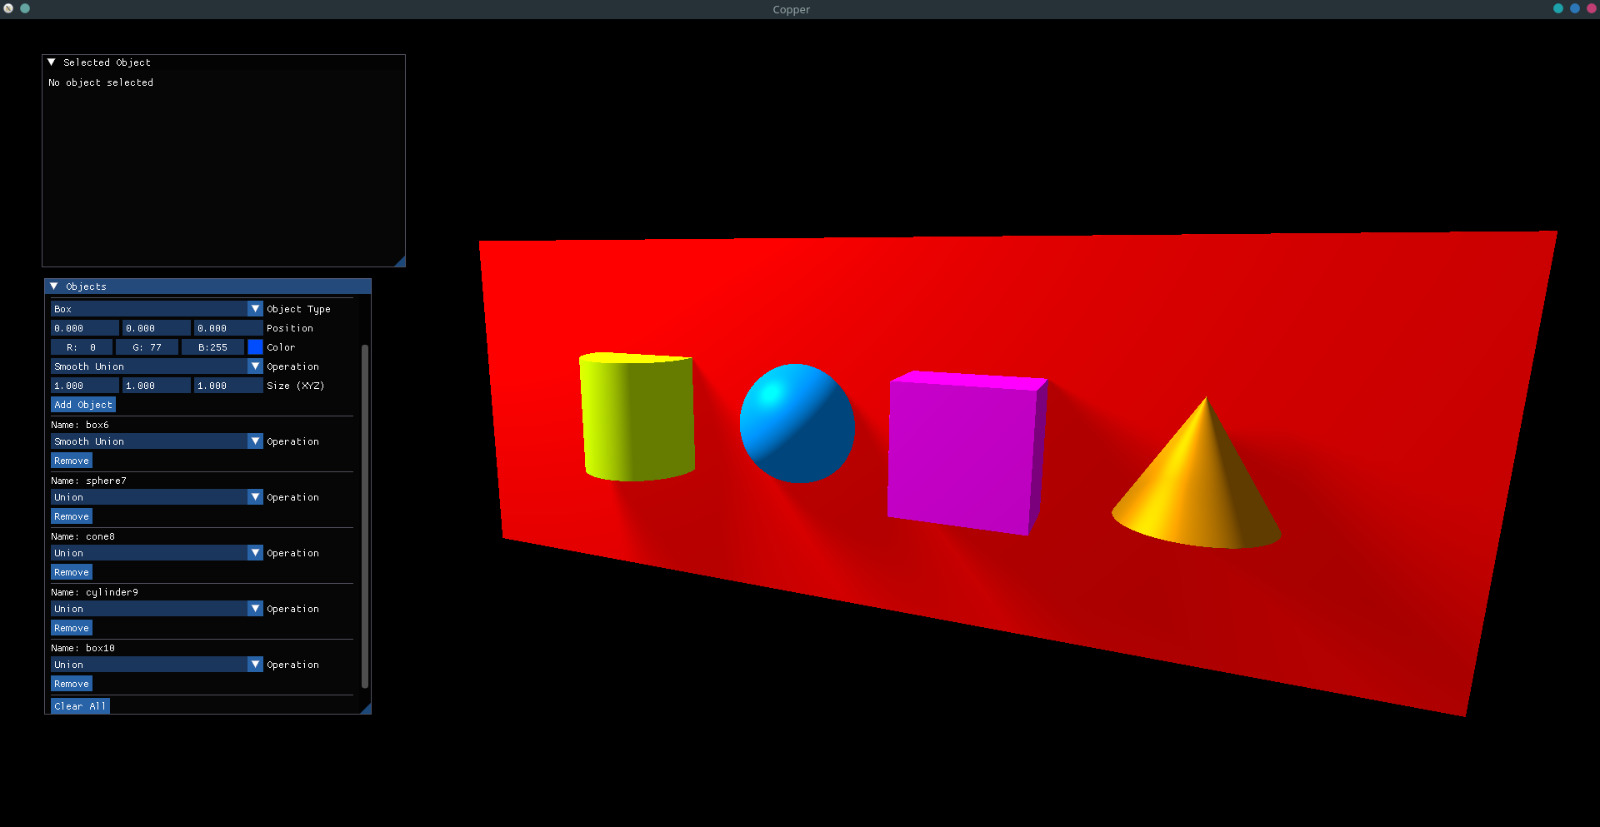
\includegraphics[width=0.7\textwidth]{imagenes/union.jpg}
	\caption{Ejemplo de operación de unión entre objetos.}
\end{figure}